\section{Overview}
\textbf{View subsystem:}
This subsystem contains the different types of views that will show, depending on how the user is 
using the system. Therefore, its assignment of functionality will be that this subsystem 
has to keep track of the different views.\\
\textbf{Model subsystem:}
This subsystem contains the data that the system will be using. When the model changes state, 
it will notify the controllers, and the controllers will then change the view. Therefore, 
this subsystems assignment of functionality will be notifying the controllers, 
when its state is being changed.\\
\textbf{Controller subsystem:}
This subsystem is being used to update the views, by receiving the models state. 
Its assignment of functionality will be that this subsystem will have to update the views 
with the received models state.\\
\textbf{DataStorage subsystem:}
The DataStorage subsystem creates persistance of data either through a Database connection or locally in a file storage. The Client can gain access to the storage through a storage client which controls which kind of storage must be used at a given time and also controls the logic for the model to storage convertion. 

\subsection{Overview of the program}
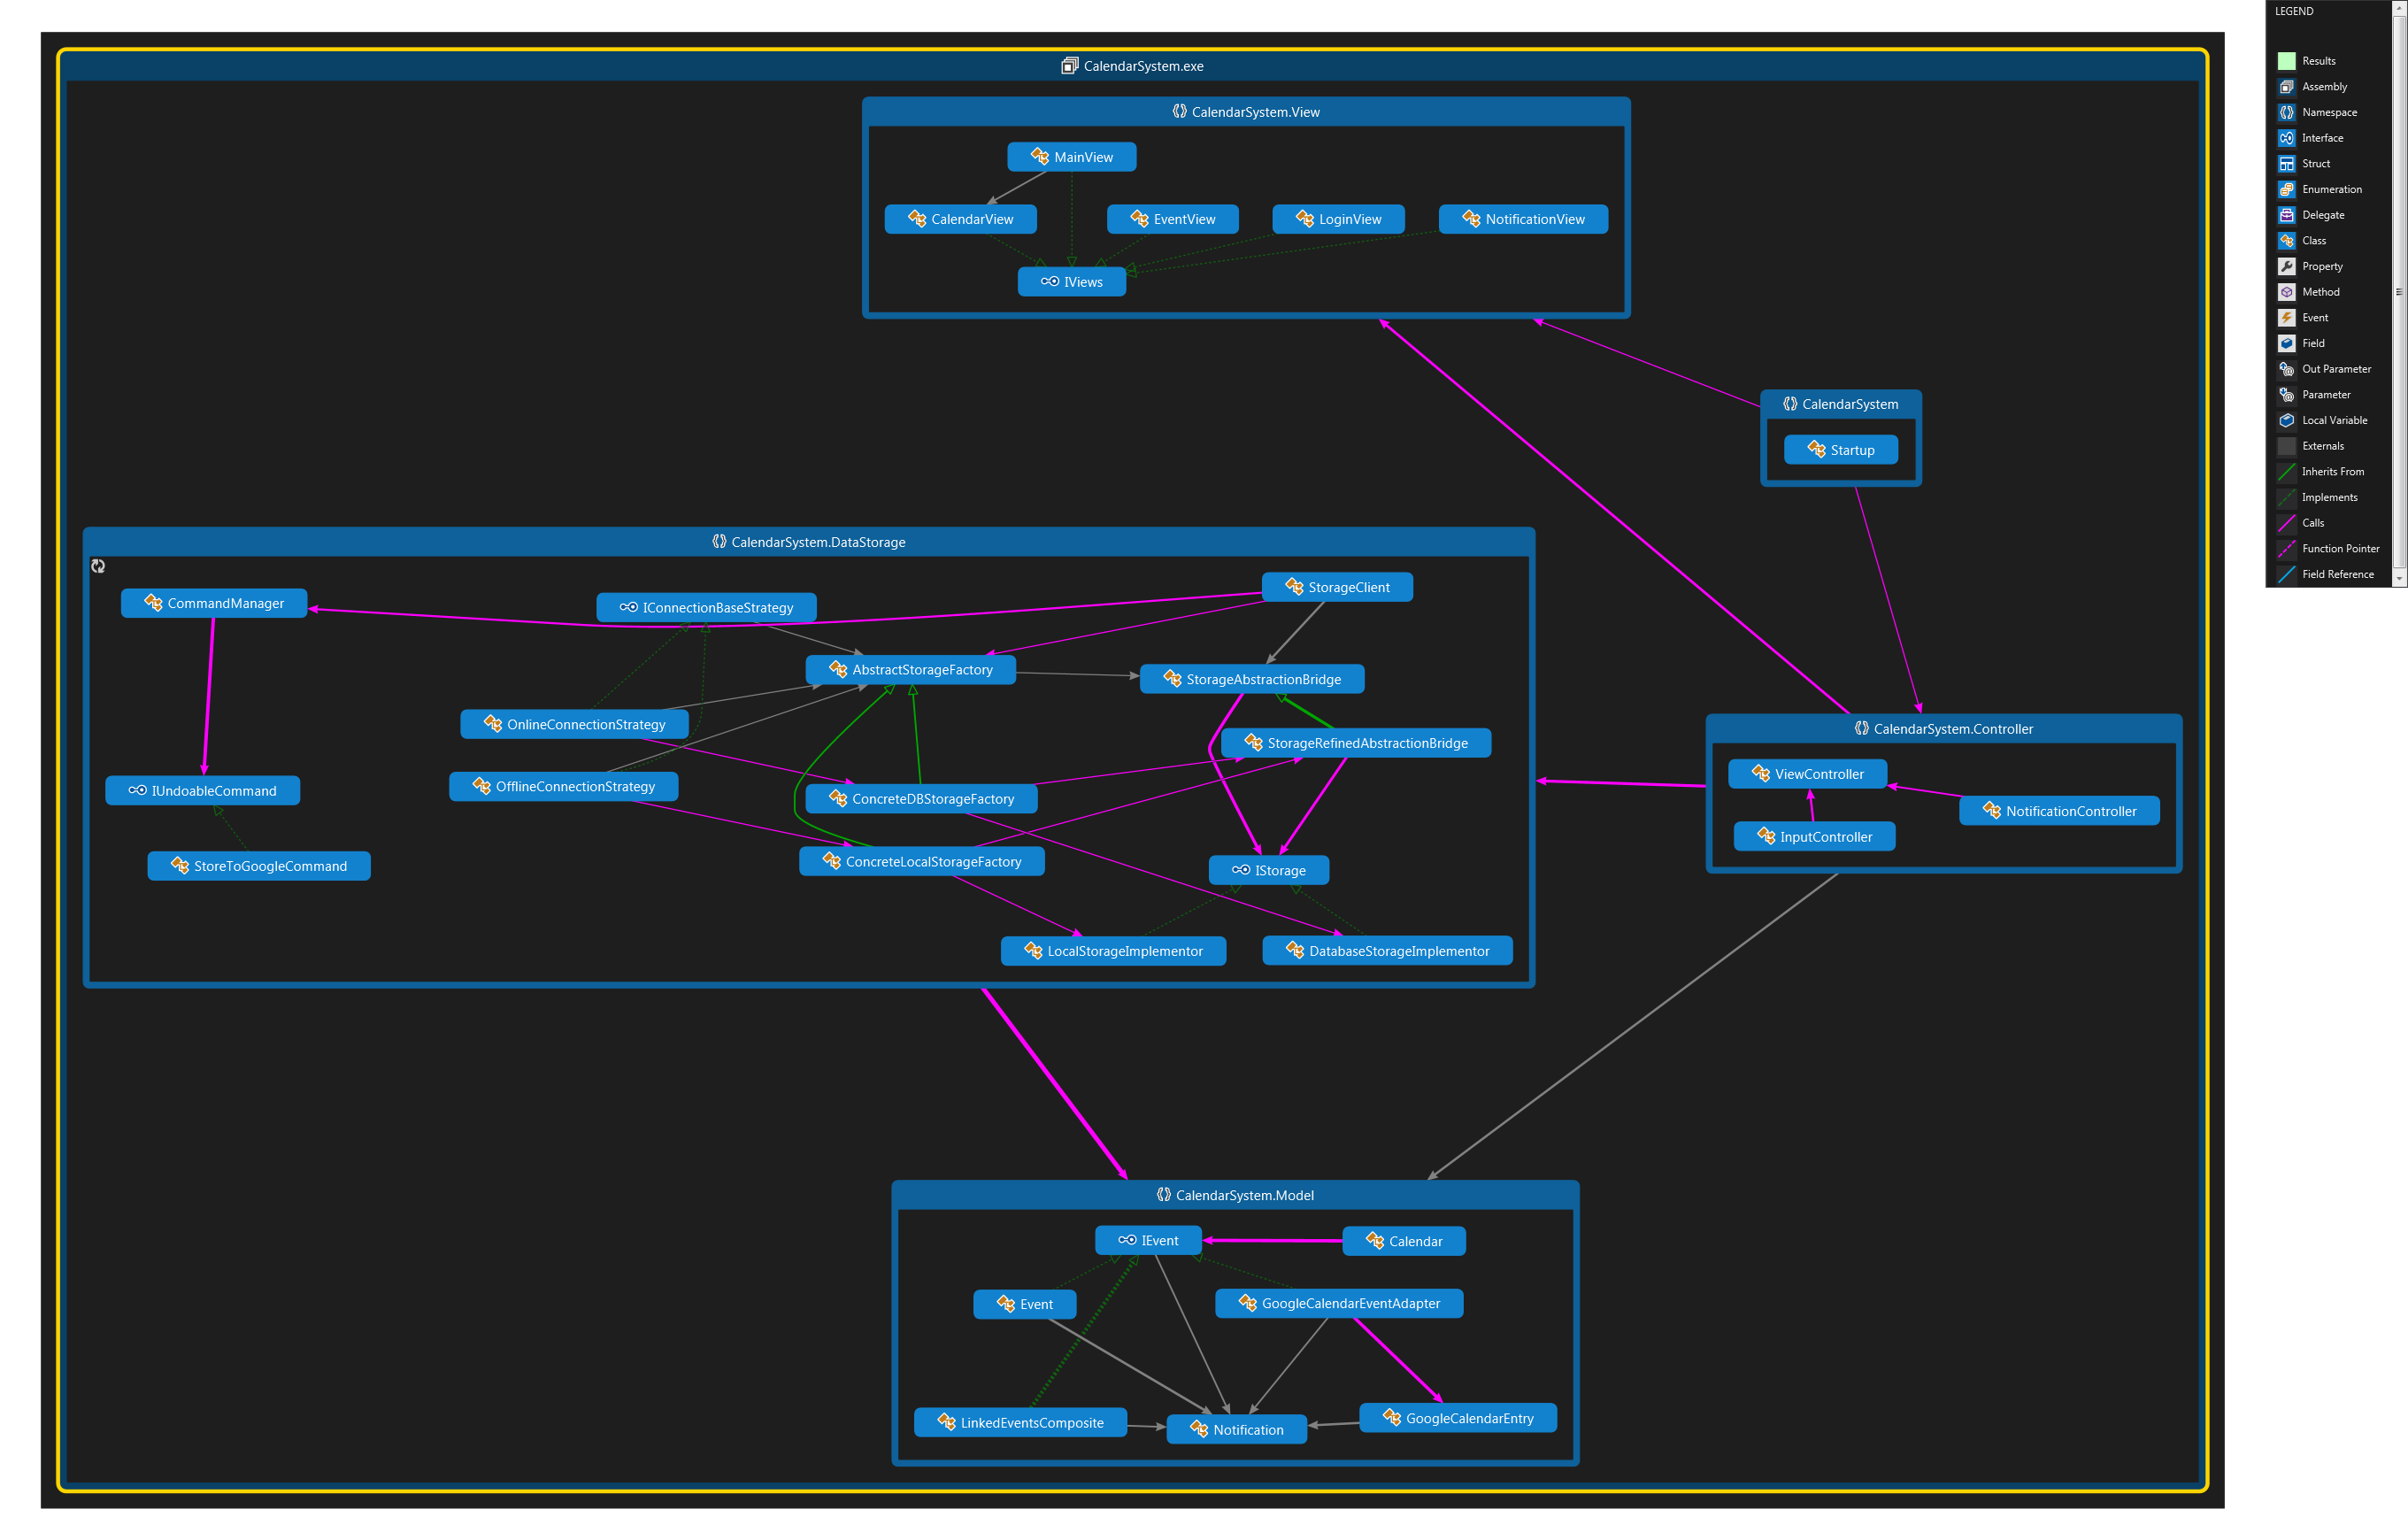
\includegraphics[scale=0.2]{OverallClassDependencies}
The figure shows the overall dependencies of the system, which object refers to which. References between objects in the subsystems are not included. In the Model Subsystem the objects form the data we want represented. Events, notifications, and so on. \\There are also a few extra classes the LinkedEventsComposite which is part of a Composite pattern used for linking together events, and the GoogleCalendarEventAdapter which is part of an Adapter pattern to make GoogleCalendarEvents able to be used along side our systems events.

The other interesting subsystem is the DataStorage. The classes of the subsystem form a number of objects which are used to store data. The objects form a number of design patterns together: The classes which is suffixed with Strategy forms a strategy pattern used to choose which factory to use. \\The classes suffixed with Factory is part of the Abstract factory pattern. These factories creates the products LocalStorageImplementor and DatabaseStorageImplementor in a bridge pattern class (suffixed with Bridge). \\The classes containing Command in their name are part of a command pattern, here the CommandManager can hold a number of commands, execute them and in case of a failure, call the commands undo method.\\

The classes in the subsystems Controller and View do not contain any design patterns.